\section{Results}

\subsection{Scenario analysis}



\begin{figure}
    \centering
    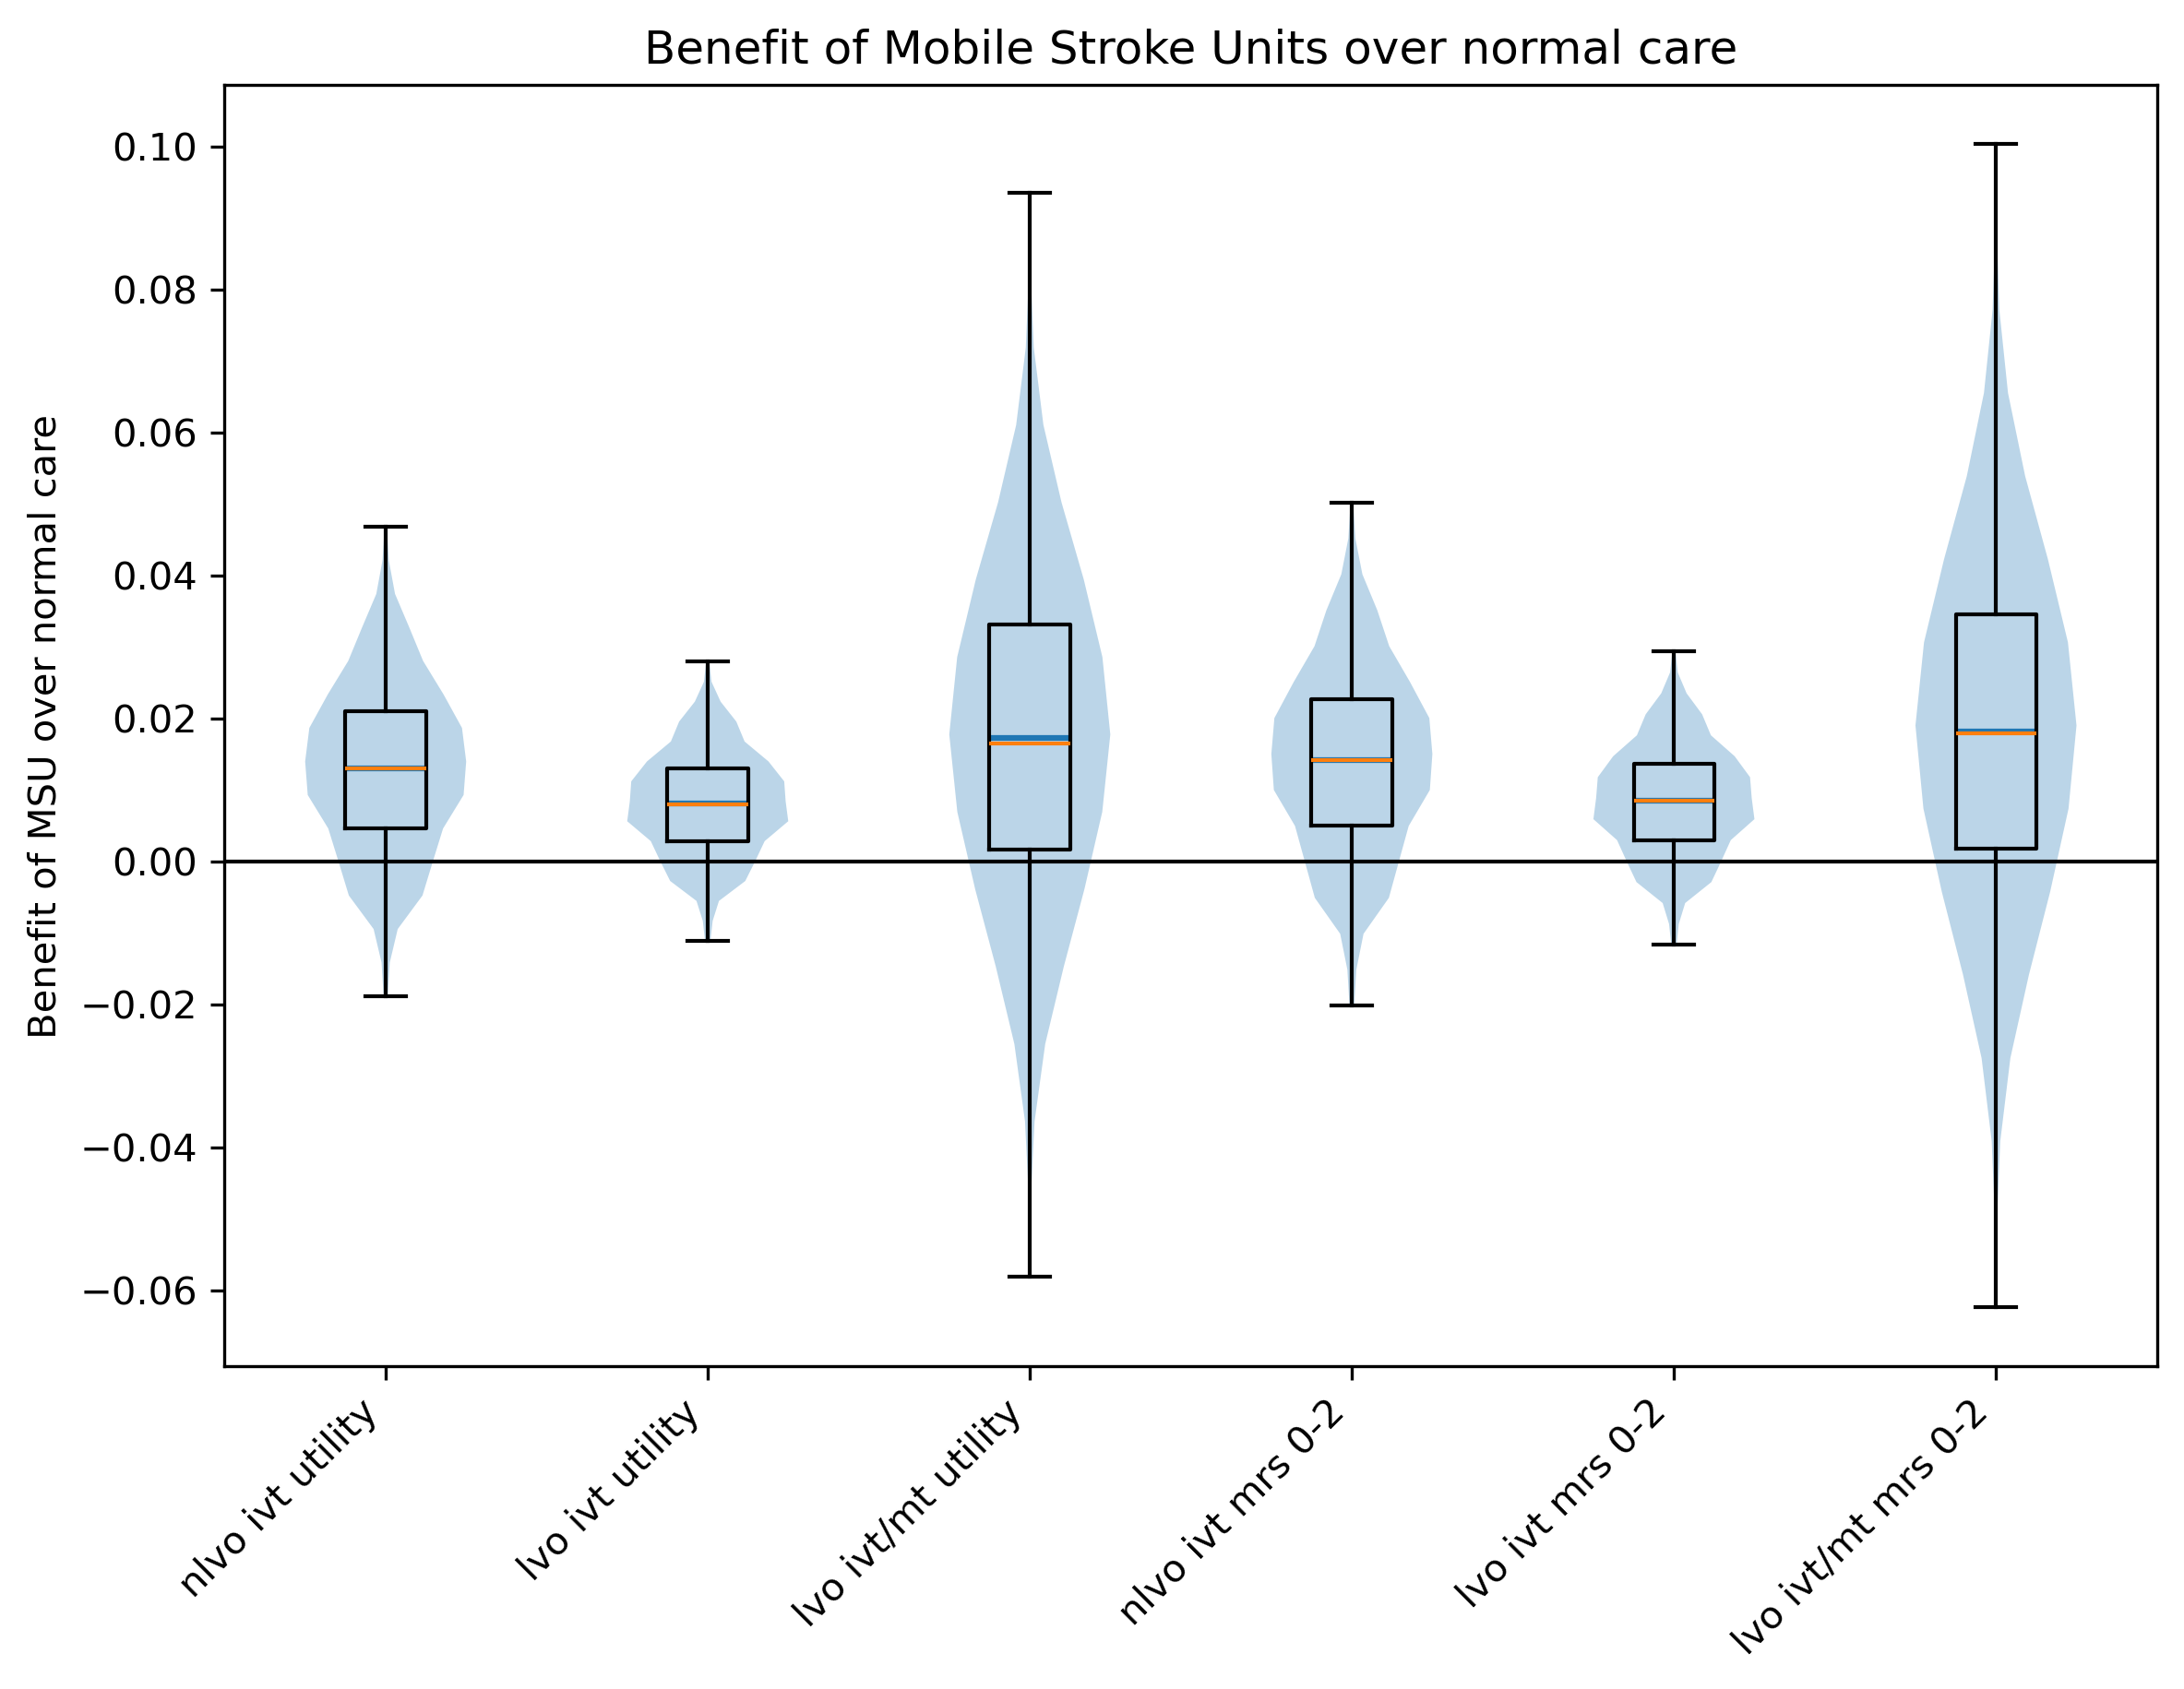
\includegraphics[width=0.6\linewidth]{images/scenario_results_summary.png}
    \caption{Enter Caption}
    \label{fig:enter-label}
\end{figure}


\begin{figure}
    \centering
    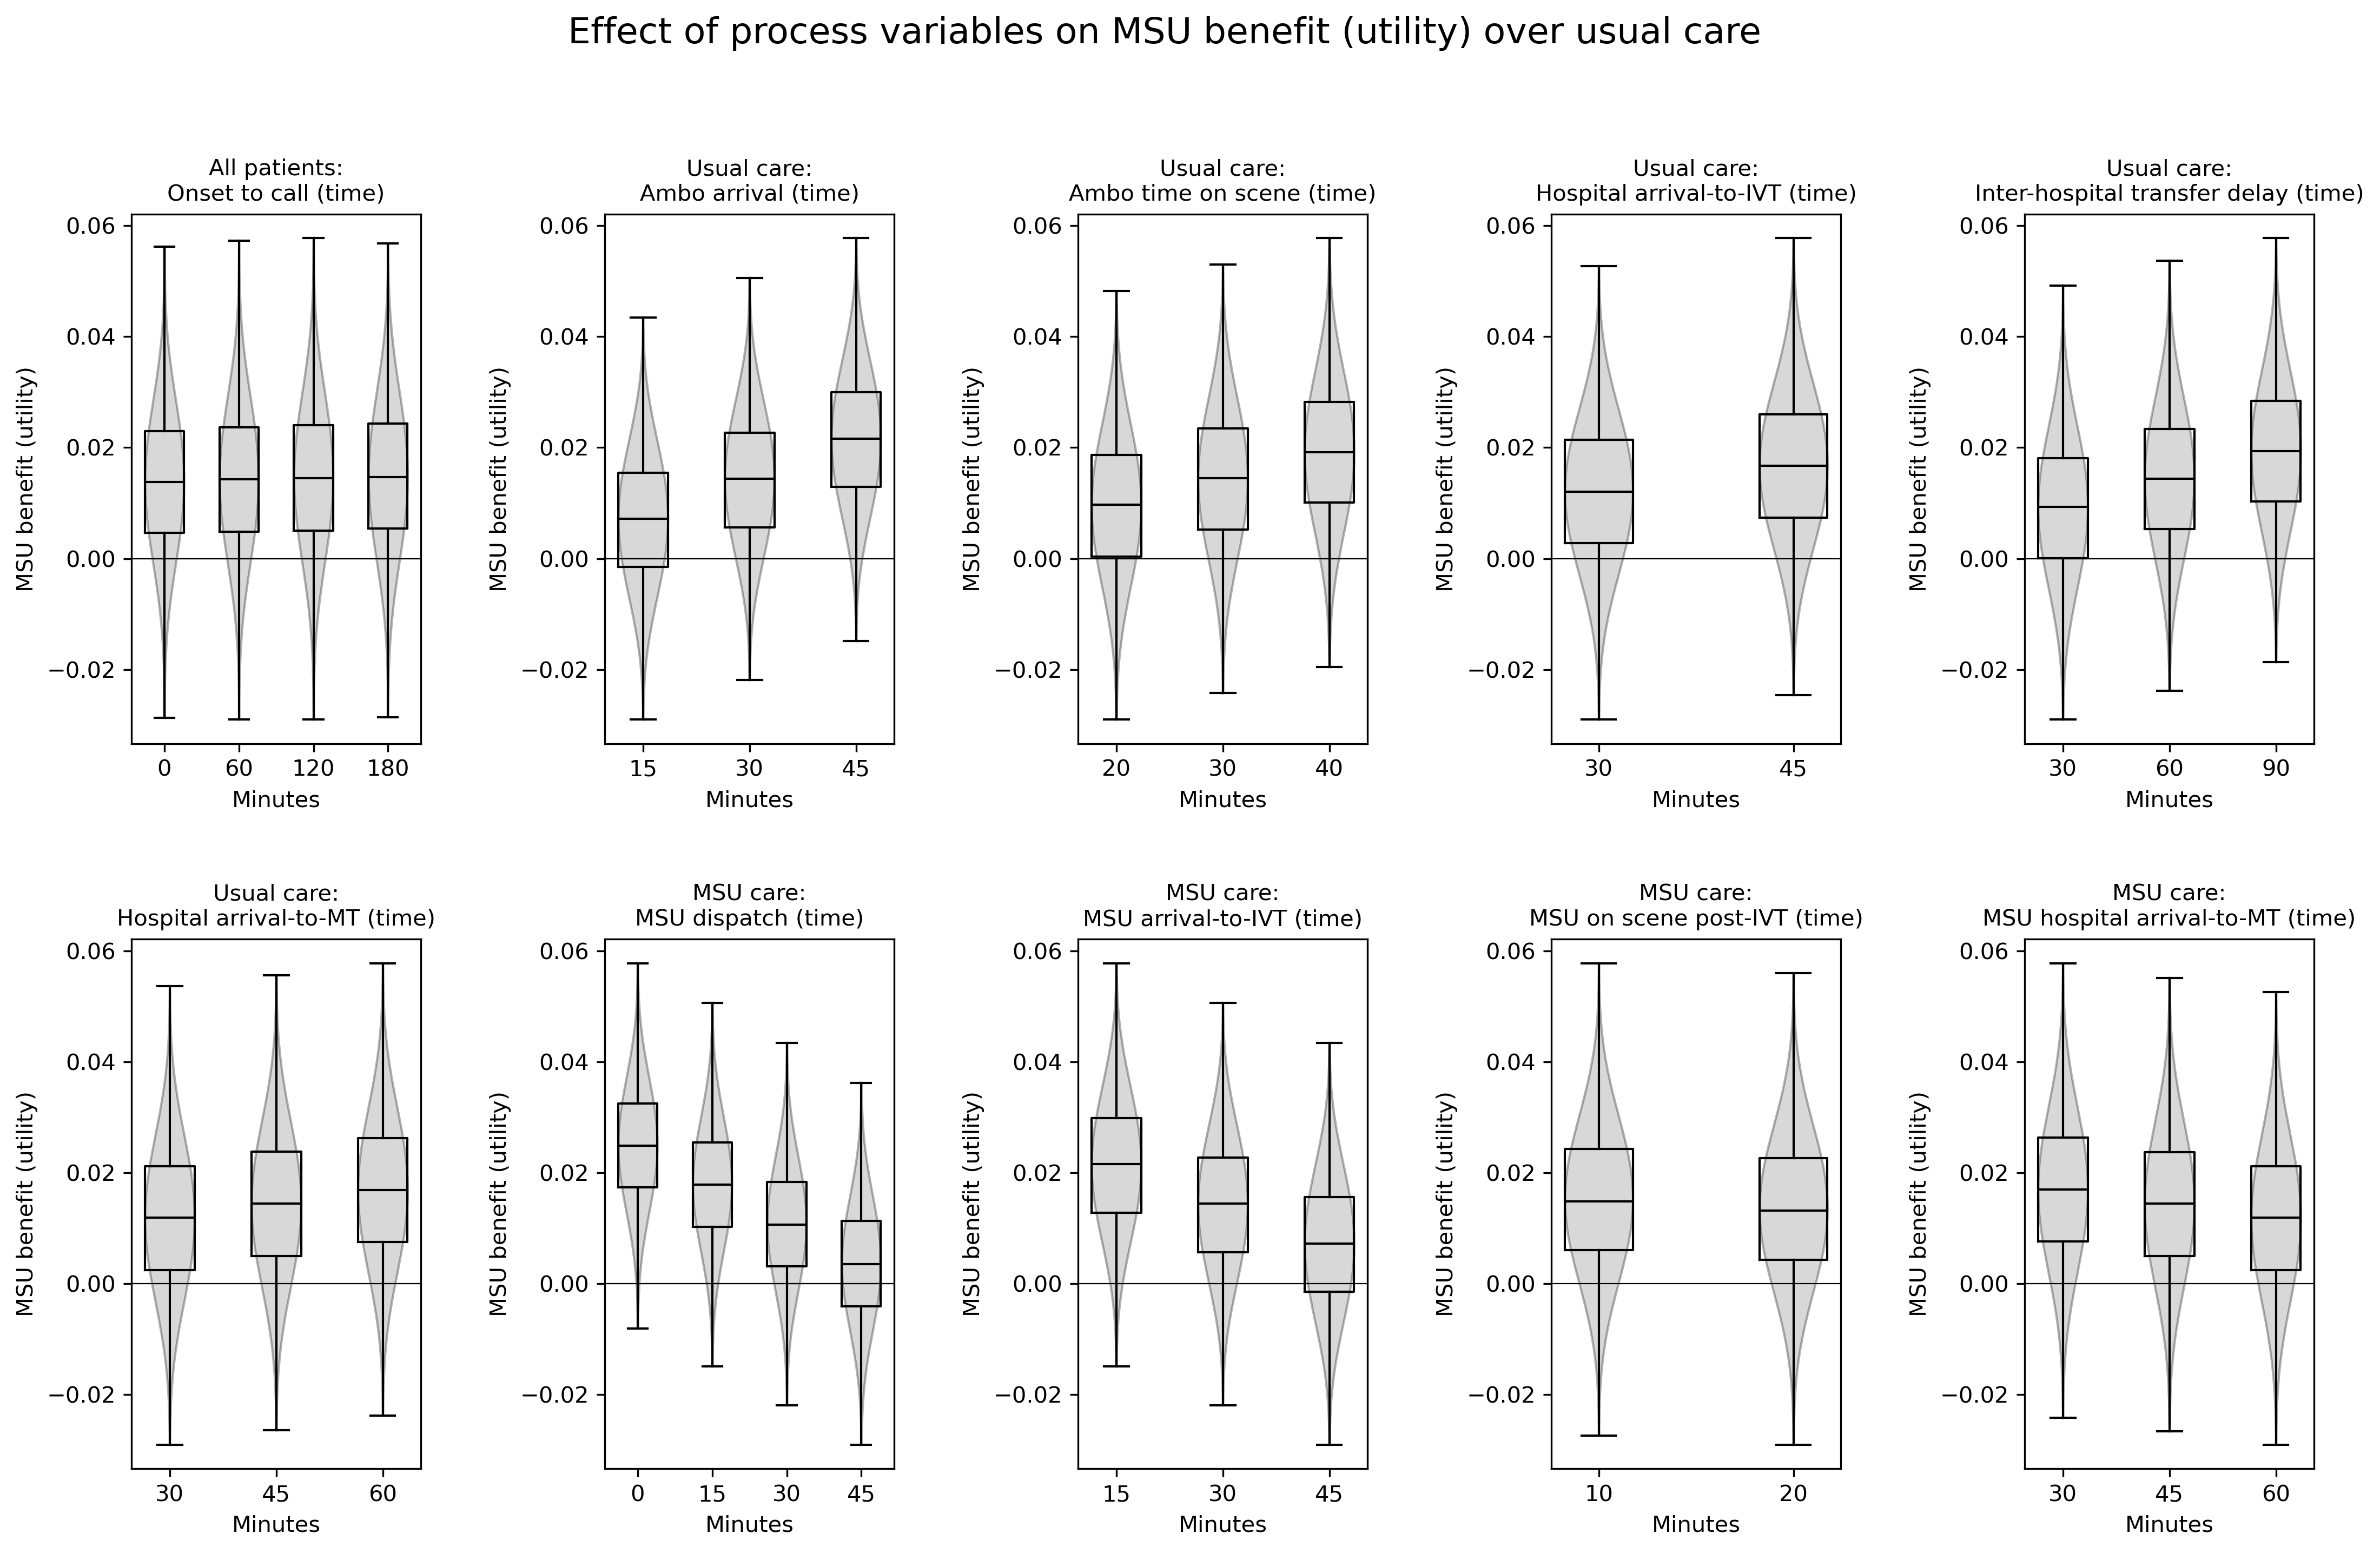
\includegraphics[width=1\linewidth]{images/msu_net_utility_benefit.png}
    \caption{Enter Caption}
    \label{fig:enter-label}
\end{figure}

\subsection{Geographic variation}


\begin{figure}
    \centering
    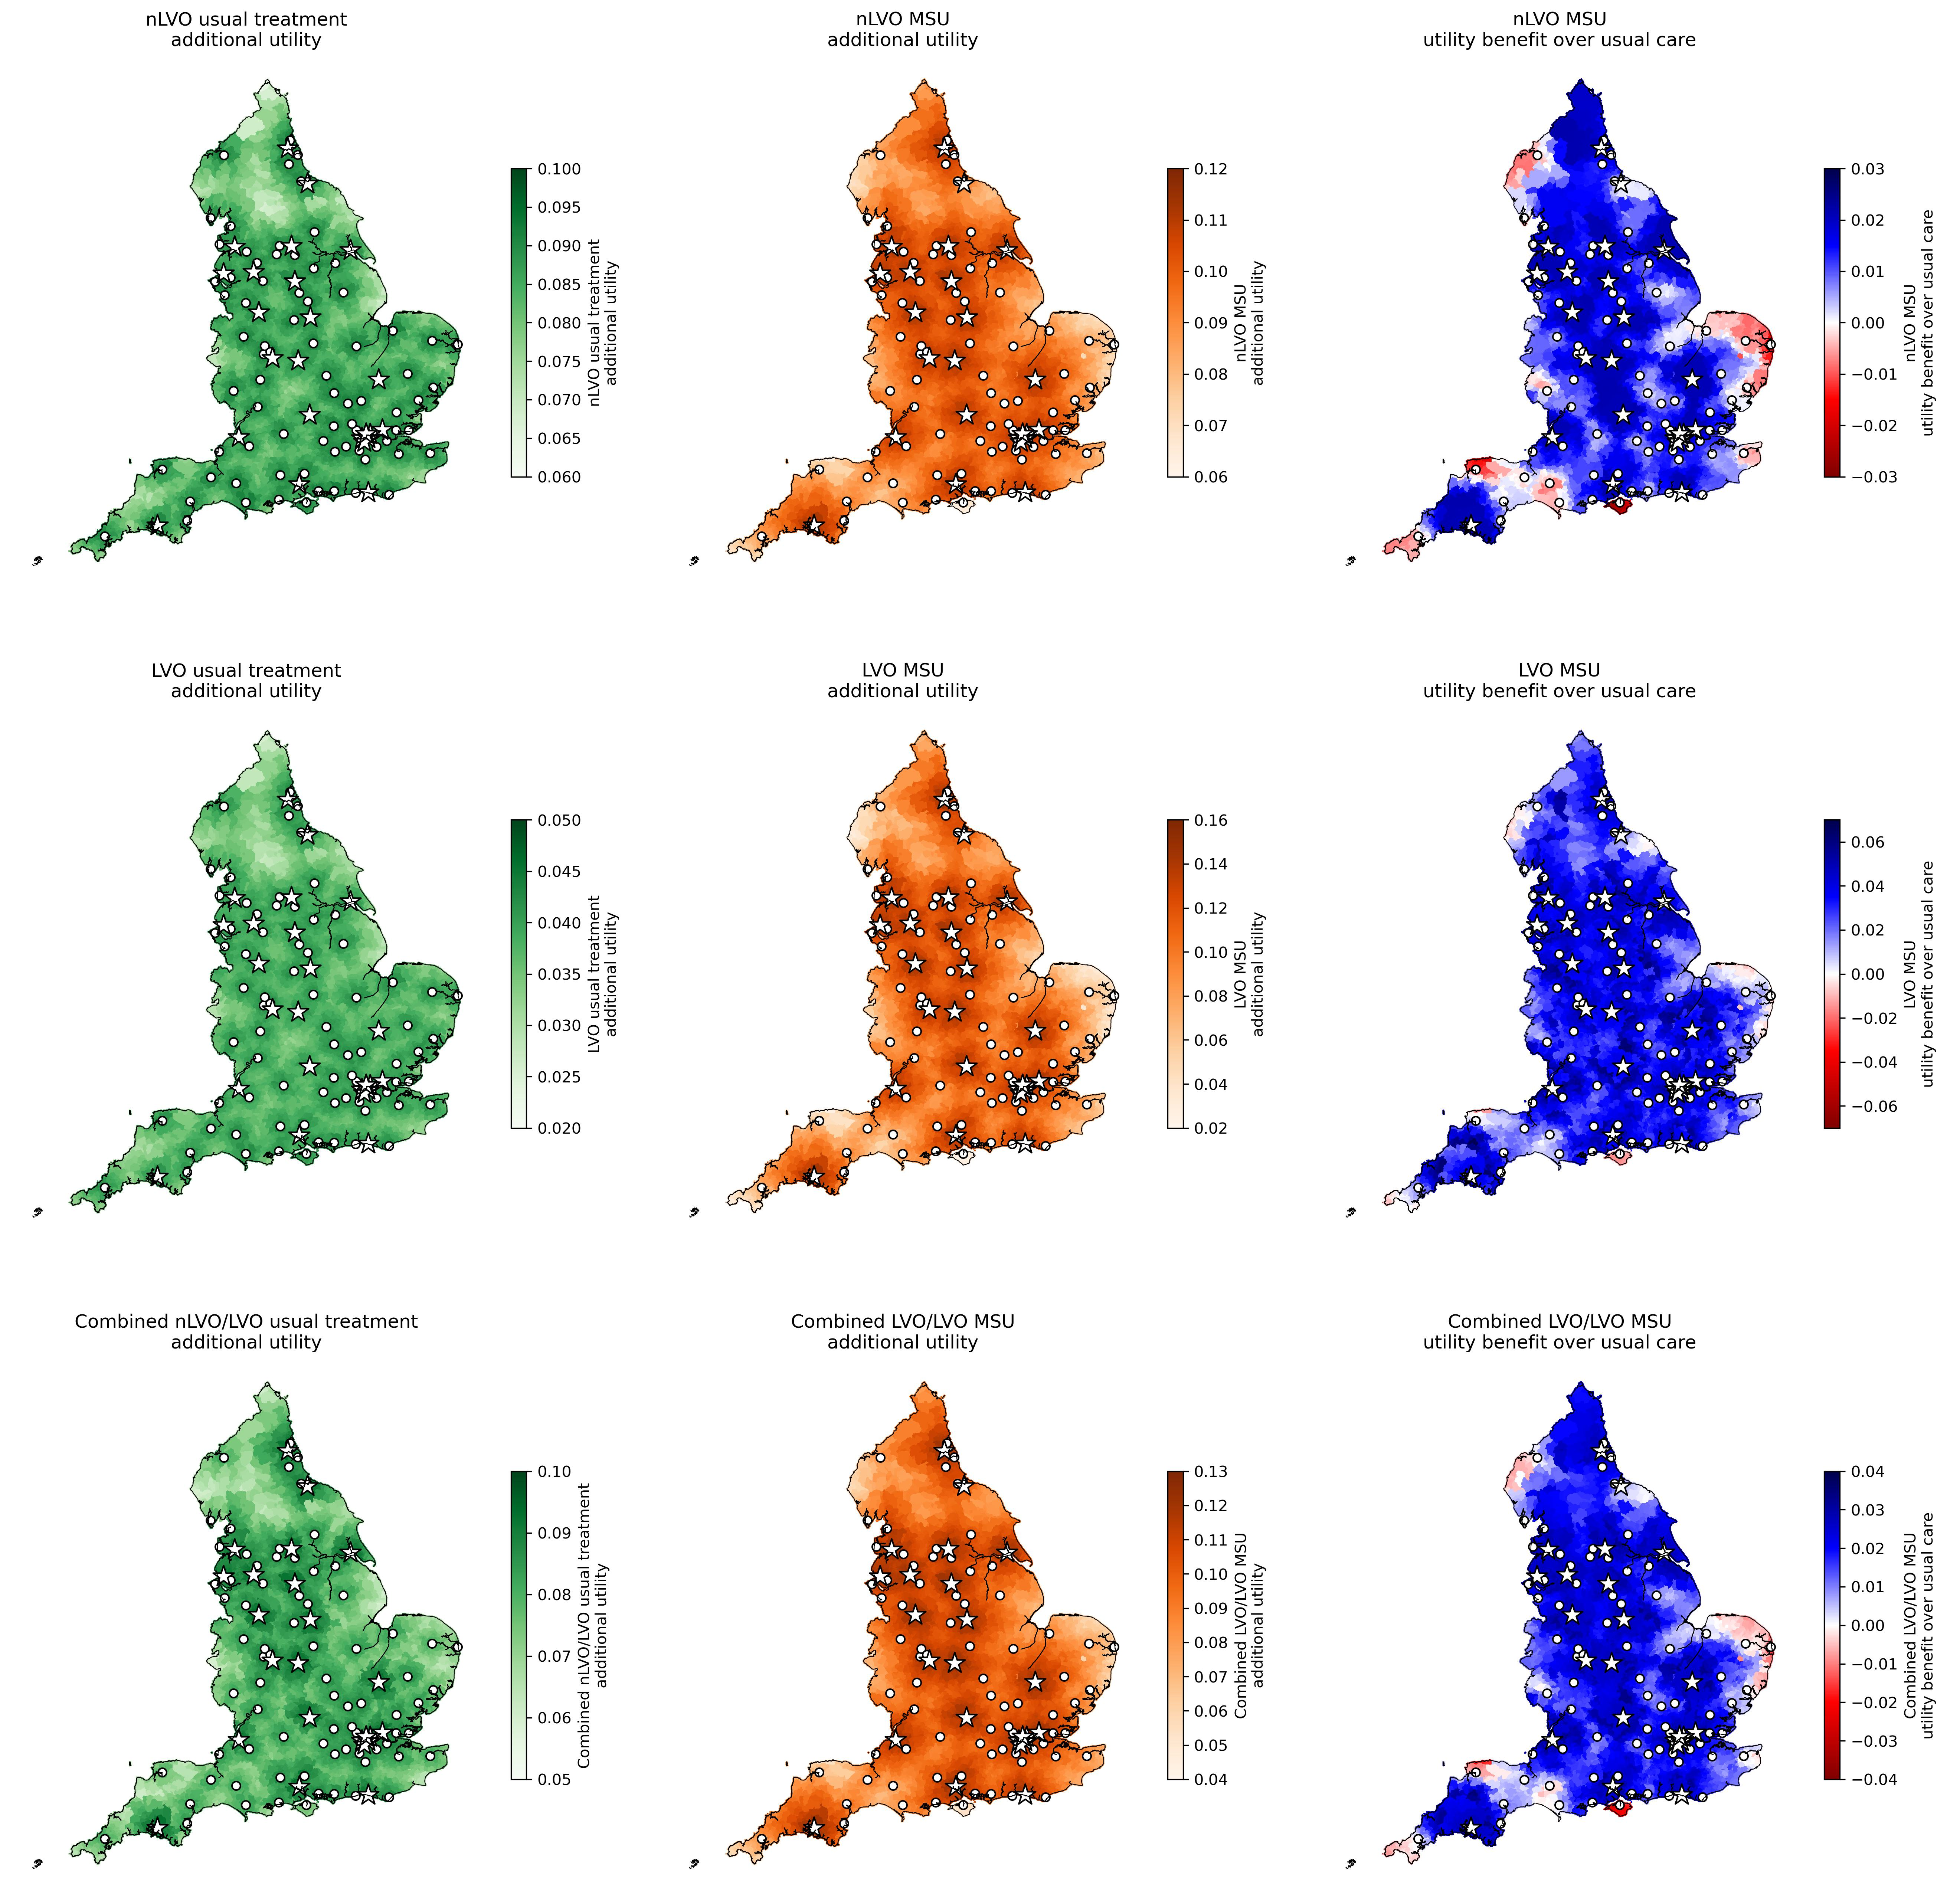
\includegraphics[width=1\linewidth]{images/map_utility.jpg}
    \caption{Enter Caption}
    \label{fig:enter-label}
\end{figure}

\begin{figure}
    \centering
    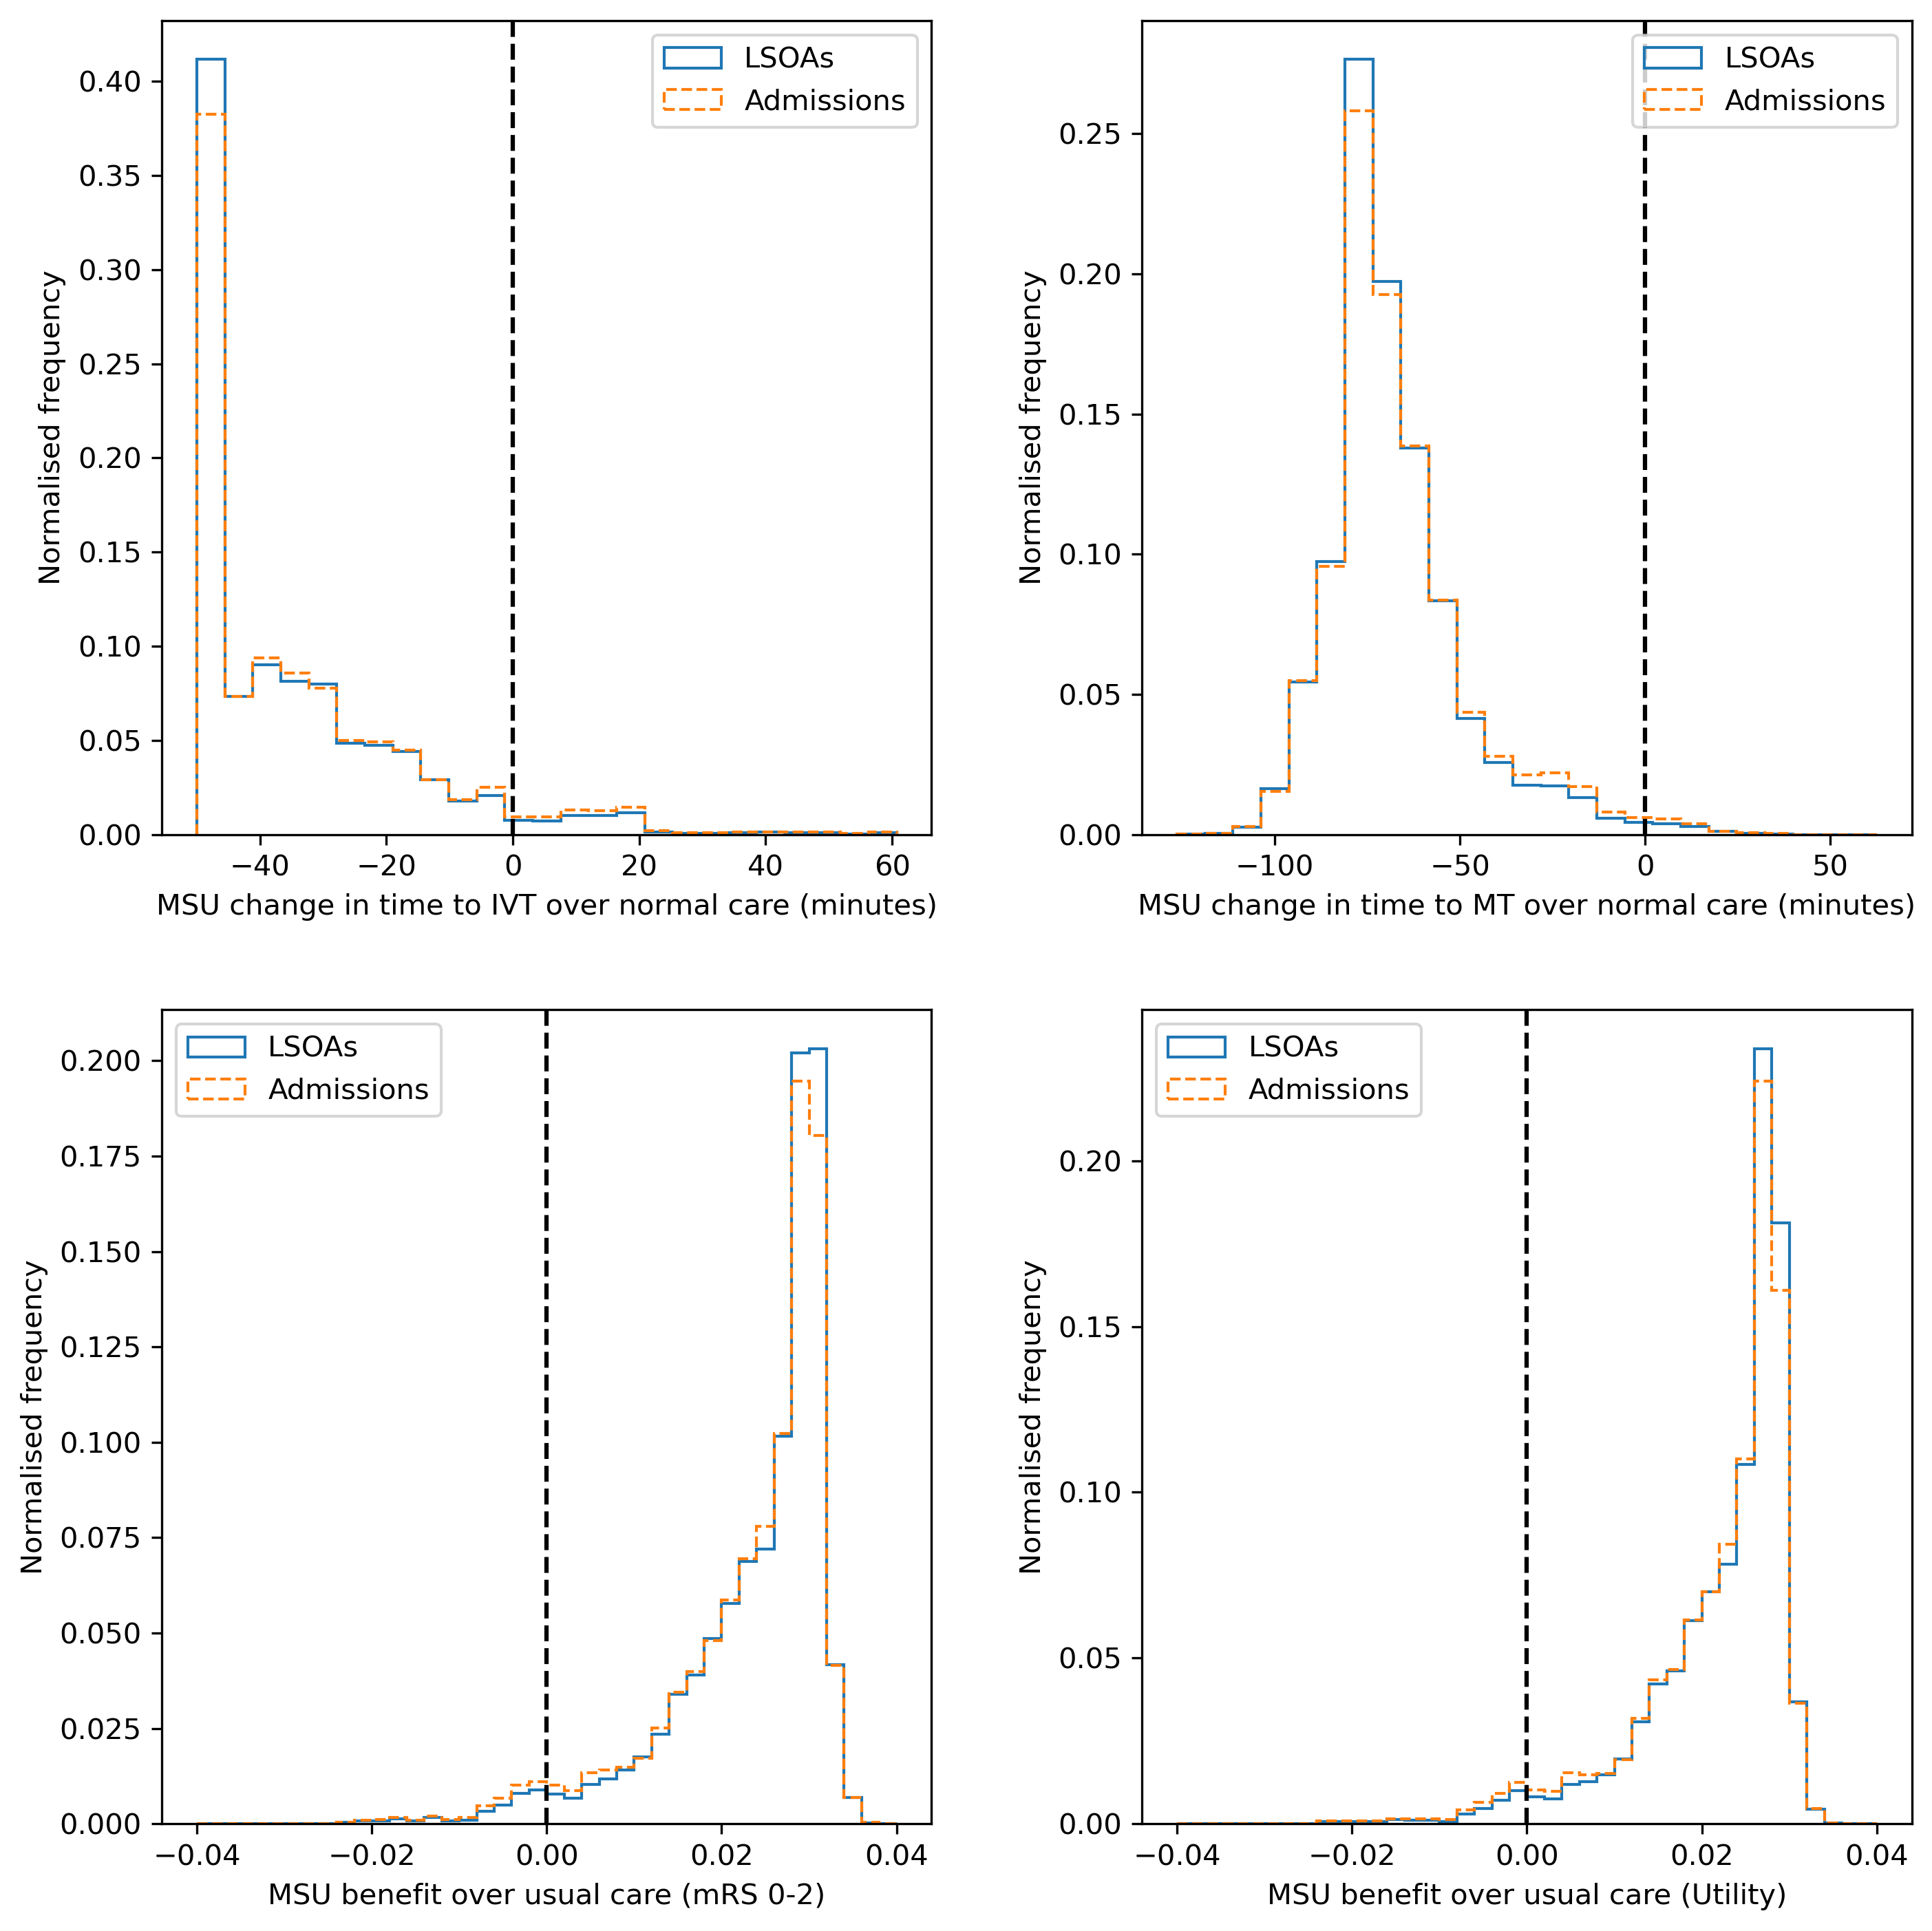
\includegraphics[width=0.75\linewidth]{images/histograms.png}
    \caption{Enter Caption}
    \label{fig:enter-label}
\end{figure}



\begin{figure}
    \centering
    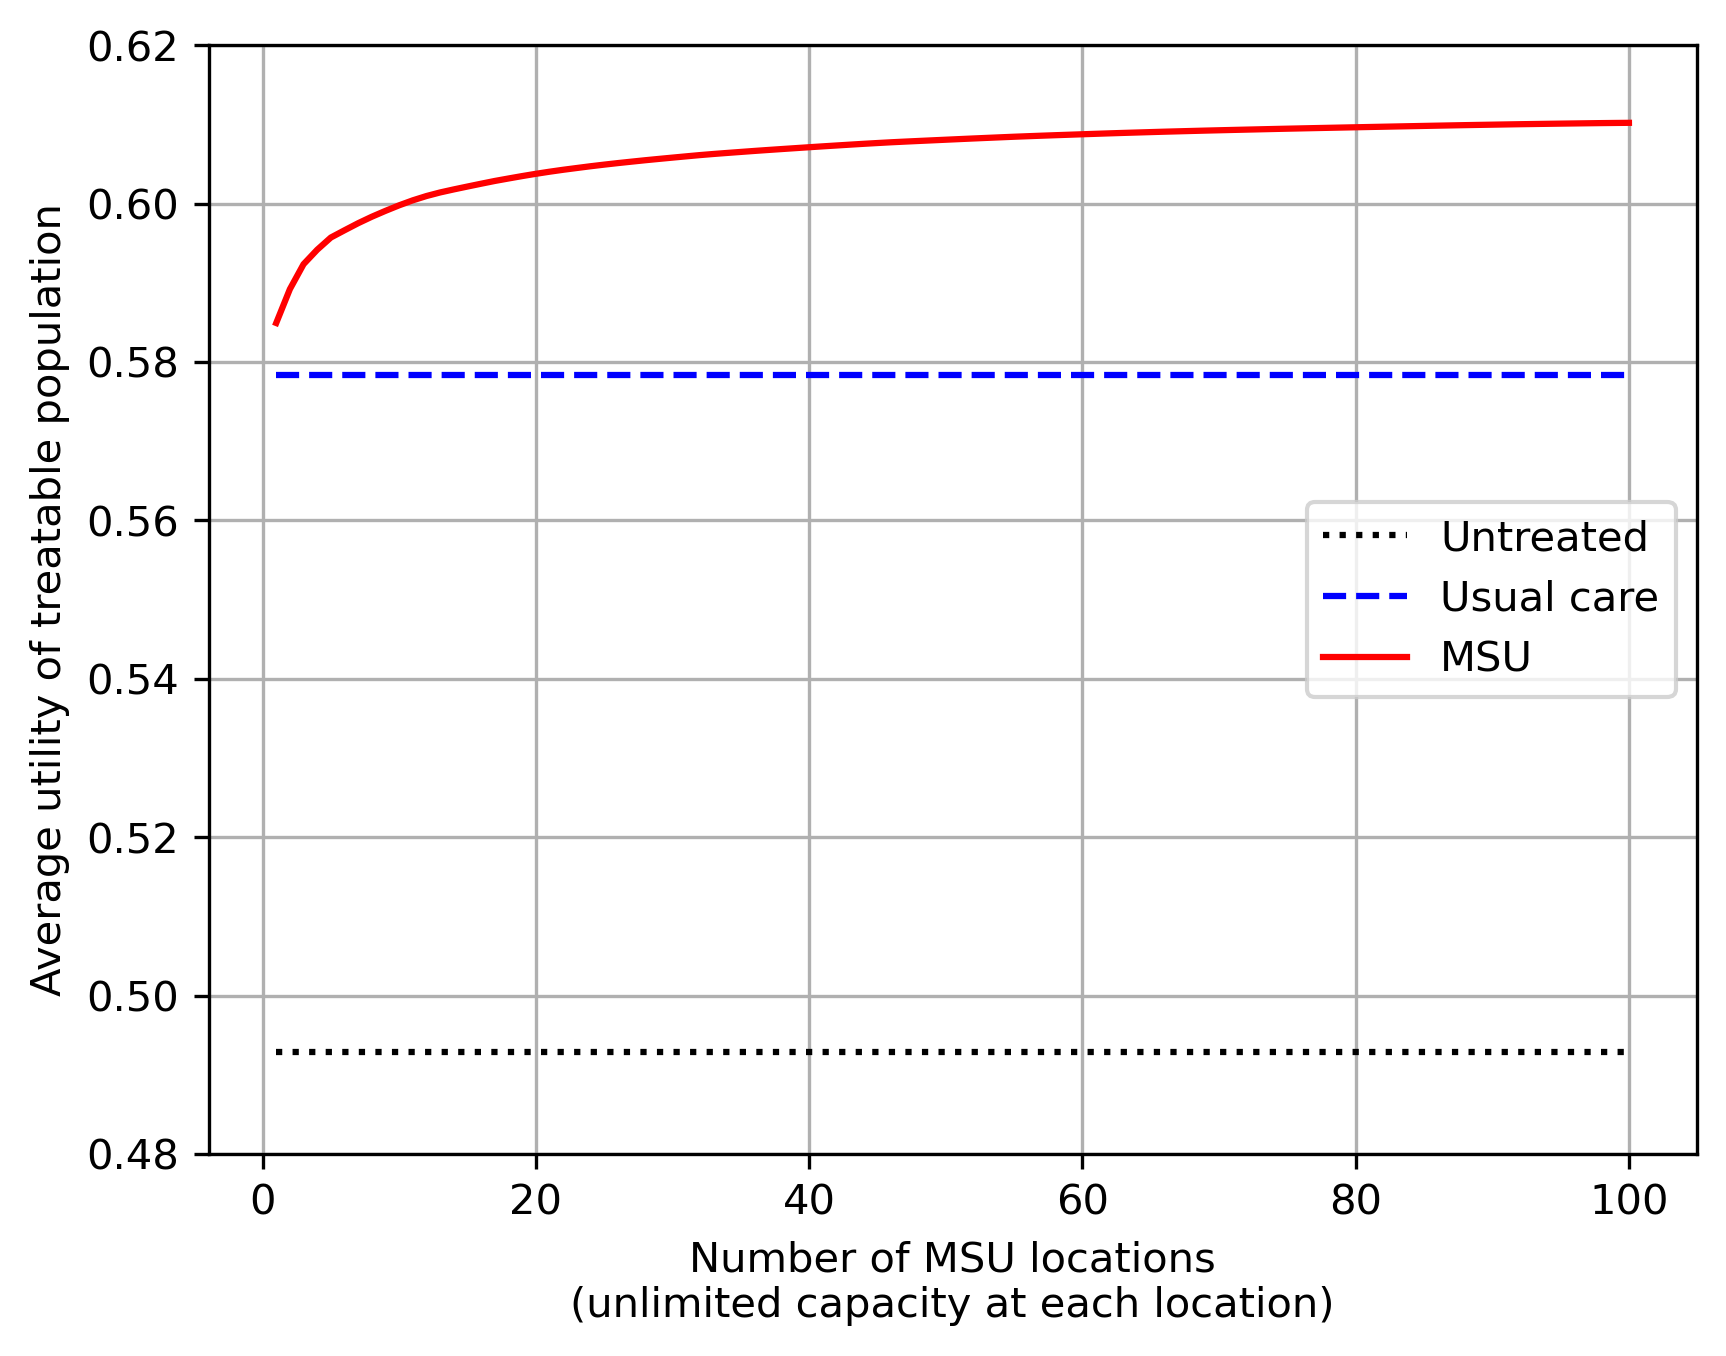
\includegraphics[width=0.5\linewidth]{images/greedy.png}
    \caption{Enter Caption}
    \label{fig:enter-label}
\end{figure}

When selecting locations of mobile stroke units, in the first 10 selections, 3 were comprehensive stroke units, and in the first 20, 7 were comprehensive stroke units.
